% !TeX root = ../main.tex
\chapter{Einleitung}\label{chap:einleitung}
\section{Ausgangslage}
Beschreibt das konkrete Problem und die Zielgruppe.
\section{Zielsetzung und Abgrenzung}
Was soll entstehen? Welche Fragen beantwortet die Arbeit?
\section{Aufgabenverteilung}
Welche Person verantwortet welchen Teil?

\begin{figure}
    \centering
    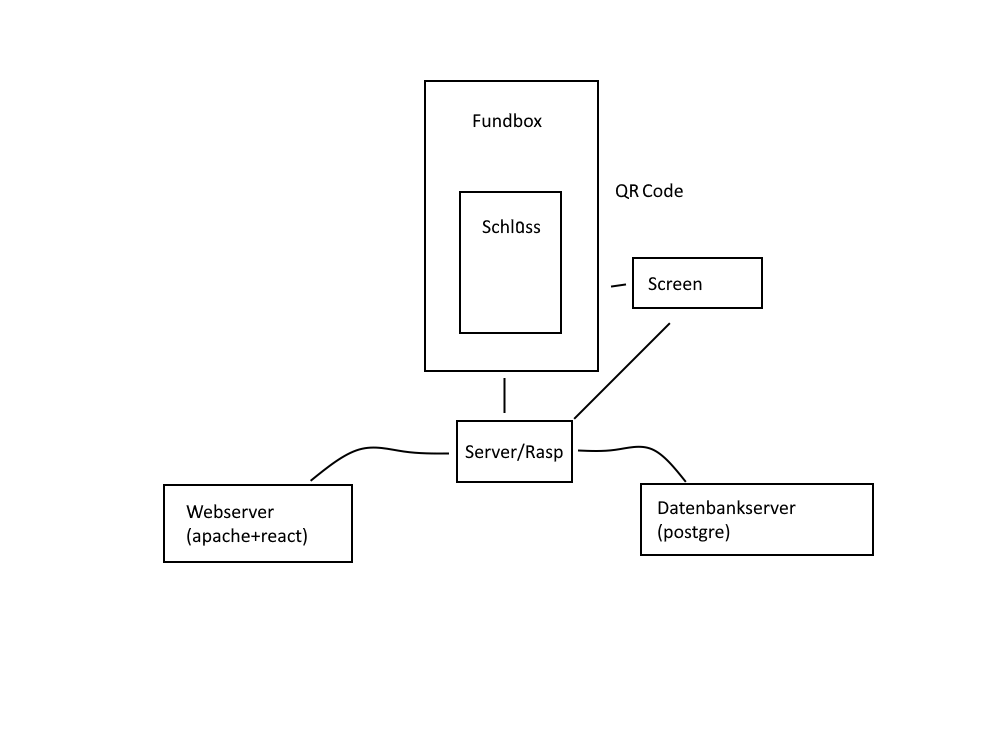
\includegraphics[width = 0.5\textwidth]
    {bilder/Components1.png}
    \caption{Komponentendiagramm}
    \label{fig.componentDiagram}
\end{figure}
